\section{Message Authentication Codes based on Hash-Functions using Merkle Trees}

To guarantee the integrity of transfered data, there is the possibility to use Merkle Trees on Message Authentication Codes (MAC) alongside hash-functions like it is described in chapter three in this paper. Merkle Trees are hash trees named after the scientist Ralph Merkle „where the value associated with a node is a one-way function of the nodes’s children. For many applications, one wishes to output a sequence of consecutive leaves (or leaf pre-images), along with their “authentication paths” – the latter consists of the interior nodes that constitute the siblings on the path from the leaf to the root. Given an authentication path and a leaf, one can verify the correctness of the latter with respect to the publicly known root value.“ \cite{MT} 

\begin{figure}
\centering
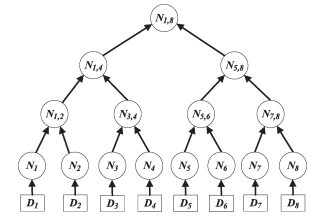
\includegraphics[width=6cm]{Pages/Merkle/merkleTree.png}
\caption{Merkle Tree Structure}
\end{figure}

In Fig 1. the data (d) is shown with the letter „D“ and the nodes are represented with the letter N. The data itself is not considered part of the Merkle Tree. The Nodes h(D\textsubscript{i})(i = 1,..., 8) are the hashed values of the data and this is where the Merkle Tree starts. Nodes in the same row are considered as siblings and the nodes above are their parents, which values are deviated from their children. Nodes without children are called leaf nodes. This hash tree is also called binary tree because every parent has two children. Binary trees have a height H with $ 2^{H} $ leaves, and $  2^{H} $ - 1 nodes. \cite{MT} 
For example the hash value of node N1,2 is h1,2 = h(h1|h1), and the hashed value of the node N1,8 is h1,8 = h(h1,4|h5,8). \cite{METR} The node on the top is also called root node and contains the final hash value. Every child node can be affirmed with the root node and its authentication path information (API). For example, the integrity of node N1 can be verified from the server that stores the hashed value h1,8 as: „N1 sends D1 and the corresponding API = h2, h3,4, h5,8 to the server. Then, the server can check the authenticity of node N1 by first computing h1, h1,2 = h(h1|h2), h1,4 = h(h1,2|h3,4), h1,8 = h(h1,4|h5,8). And then, the server checks whether the computed h1,8 is the same as the existing h1,8“. \cite{METR} N1 will only be accepted by the server, if both values are the same. So that means that you can look at a part of a file to check if this is correct without having the entire thing available.

\subsection{Outcome and hashing}
To hash the data you have to choose a function that is able to do this. One choice would be, for example, SHA-1 with a length of 128 bit.
„The value of a leaf, in turn, is a one-way function of some leaf preimage. For small trees these pre-images may be simply stored; alternatively for larger trees, the leaves may be calculated with a keyed pseudorandom generator.“ \cite{MT} Because the hash functions are the only thing that have to be computed, the computation time, regarding the verification, is quite low. \cite{METR} In a Merkle Tree structure it is desired to generate an output sequence fore every leaf that has two components; the leaf pre-image, and the authentication path (Fig 2) \cite{MT}

\begin{figure}
\centering
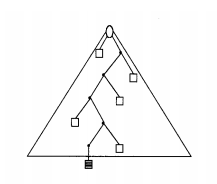
\includegraphics[width=5cm]{Pages/Merkle/API.png}
\caption{Authentication Path}
\end{figure}

The circle in Fig. 2 represents the root node; the grey square is the leaf’s pre-image, and the white squares biuld the authentication path of the grey square.

\subsection{Security and speed}
„Since software implementations of hash functions are much more efficient than software implementations of finite field arithmetic, the Merkle signature scheme (MSS) is a good candidate for implementations on small microprocessors without cryptographic coprocessors“. \cite{FHB} Like mentioned before, the hash function is the only thing that has to be computed and so it is inportant to choose a propper one regarding to it’s cryptographic properties because MSS relies only to it. So that is on the one hand a big benefit and on the other hand a disadvantage if it is found insecure. But if the hash function appears to be insecure, it can be easily replaced with a secure one to make the MSS save again. Also the signature generation is faster than RSA and comparable to ECDSA. Further performance improvements are reached by utilizing a symmetric crypto engine such as an AES hardware acceleration. \cite{FHB}  "The total space
required is bounded by $ 1.5 log^2 $  N/loglog N hash values, and the worstcase computational effort is 2 log N/loglog N hash function evaluations
per output." \cite{MT}
